\documentclass{article}
\usepackage{amsmath}
\usepackage{amssymb}
\usepackage{graphicx}
\usepackage{enumitem}
\usepackage[utf8]{inputenc}
\usepackage{xcolor}

\graphicspath{{/home/stephanie/Escritorio/THC/Taller-de-Herramientas-Computacionales/Clases/Latex/Imagenes/}}

\title{\Huge Taller de Herramientas Computacionales}
\author{Stephanie Escobar Sánchez}
\date{23/enero/2019}


\begin{document}
	\maketitle
	\begin{center}
		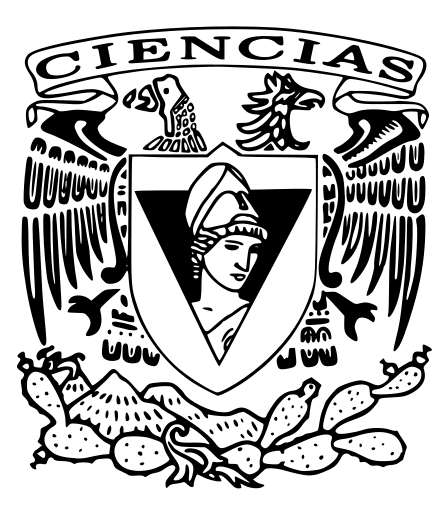
\includegraphics[scale=0.40]{1.png}	
	\end{center}
	\newpage
	\begin{center}
		\title {\textcolor{green}{\Huge \textbf{Bitácora clase 13}} }  
	\end{center}

\section{Recursividad}

Comenzamos la clase revisando unos problemas sel libro python fácil, del cuál se desplegaron muchas dudas sobre cómo resolverlos. El problema de la clase fue hacer un laberinto, en el cual debíamos saber como hacerle para dar un paso y para hacer el laberinto desde cero. Toda la case tratamos de resolver el problema del laberinto con información que ya sabíamos, como las listas, los llamados a las listas y el comando \textbf{if} y \textbf{else}.\\

Las funciones recursivas se componen de dos elementos: bases recursivas y regla de recursividad que va a generar los términos recursivos.\\
La sucesión de Fibonacci va dececiendo.
La recursividad es cuando se procesa una lista y luego se hace un llamado a las funciones faltantes estas son subrutinas y procedimientos.\\
\\
\section{Ámbitos de validez}

Los objetos de clasifican de acuerdo a su ámbito de validez que significa donde son visibles las variables. A las variables se les asigna un objeto, las variables locales solo existen mientras haga un llamado a la función (mientras se está ejecutando), las locales siempre están presentes.\\
Los ámbitos de validez se refieren a dos ticos de variables (en qué ambitos son validas)
Para evitar confusiones se agrega la palabra reservada \textit{global} para marcar cual es la variable.
También es importante etiquetar las variables de forma explícita para evitar confusiones.




\end{document}

	
